%% ----------------------------------------------------------------------------
% BIWI SA/MA thesis template
%
% Created 09/29/2006 by Andreas Ess
% Extended 13/02/2009 by Jan Lesniak - jlesniak@vision.ee.ethz.ch
%% ----------------------------------------------------------------------------
\newpage
\chapter{Related Work}
\section{Latent Variable Models}
Latent variable models are generative models which assume that it is possible to model the true data distribution $p(x)$ as a joint distribution $p(x,z)$, where $x$ and $z$ are multi-variate random vectors.
\begin{equation}
    \label{eq:marginallikelihood}
    p(x) = \int p(x,z)dz = \int p(x|z)p(z)dz
\end{equation}
Many naturally occurring distributions of samples can be imagined to come from a much simpler underlying distribution, which is obscured by the space that they are observed in. This is the main motivation behind latent variable models and in order to understand these models, it is important to define the terms used in the next sections, since they all stem from Bayesian statistics. The Bayesian theorem can be written as
\begin{equation}
    \label{eq:bayestheorem}
    p(z|x) = \frac{p(x|z)p(z)}{p(x)}
\end{equation}
which is a generally applicable formula for any conditional distributions, but in generative modeling and machine learning it is usually assumed that the letter $z$ represents a random vector of a simpler distribution in the latent (unobserved) space, and $x$ is the random vector modeling the complicated distribution in the observed space (the sample space). The four terms in the formula use distinct names:
\begin{description}
    \item[$p(x)$] is called the \textit{evidence} or the \textit{marginal likelihood}. It encompasses the actual observations of the data.
    \item[$p(z)$] is called the \textit{prior}, since it exposes information on $z$ before any conditioning.
    \item[$p(z|x)$] is called the \textit{posterior}. It describes the distribution over $z$ after (\textit{post}) having seen the evidence $x$.
    \item[$p(x|z)$] is called the \textit{likelihood}, since it gives the likelihood of observing an example $x$ when choosing the latent space to be a specific $z$.
\end{description}

\subsection{Variational Autoencoders}
One of the most straightforward examples of a generative model, where the goal is to find such a latent space representation of the training sample distribution, is the Variational Autoencoder (VAE)~\autocite{kingma2013autoencoding}. For the two factors in Eq.~\ref{eq:marginallikelihood}, the VAE uses a simple multivariate distribution as the latent $p_{\theta_z}(z)$ (e.g. a multivariate Gaussian) and a neural network mapping $p_{\theta_{NN}}(x|z)$. Training then includes finding optimal parameters for the parameterized latent distribution and for the neural network mapping, such that sampling $z$ and mapping it to the sample space is almost the same as sampling $x$ directly. When no prior over the parameters $\theta_z, \theta_{NN}$ is considered, this is usually done through an MLE (maximum likelihood estimate) $\hat{\theta} = \argmax_{\theta} p_{\theta}(x)$. While simple latent variable models can be optimized through differentiation, or iterative algorithms such as EM (expectation maximization) and gradient descent, these algorithms usually don't work for complicated multi-modal distributions (as parameterized by neural networks), since the integral in Eq.~\ref{eq:marginallikelihood} has no closed form solution and is also difficult or costly to estimate. Therefore it would be preferred to use a parameterization instead that also uses an estimation of the posterior $p_{\theta}(z|x) \approx p(z|x)$.
\begin{equation}
    \label{eq:likelihoodvae}
    p_{\theta}(x) = \int p_{\theta_{NN}}(x|z) p_{\theta_z}(z) dz
\end{equation}
\begin{figure}[h]
    \centering
    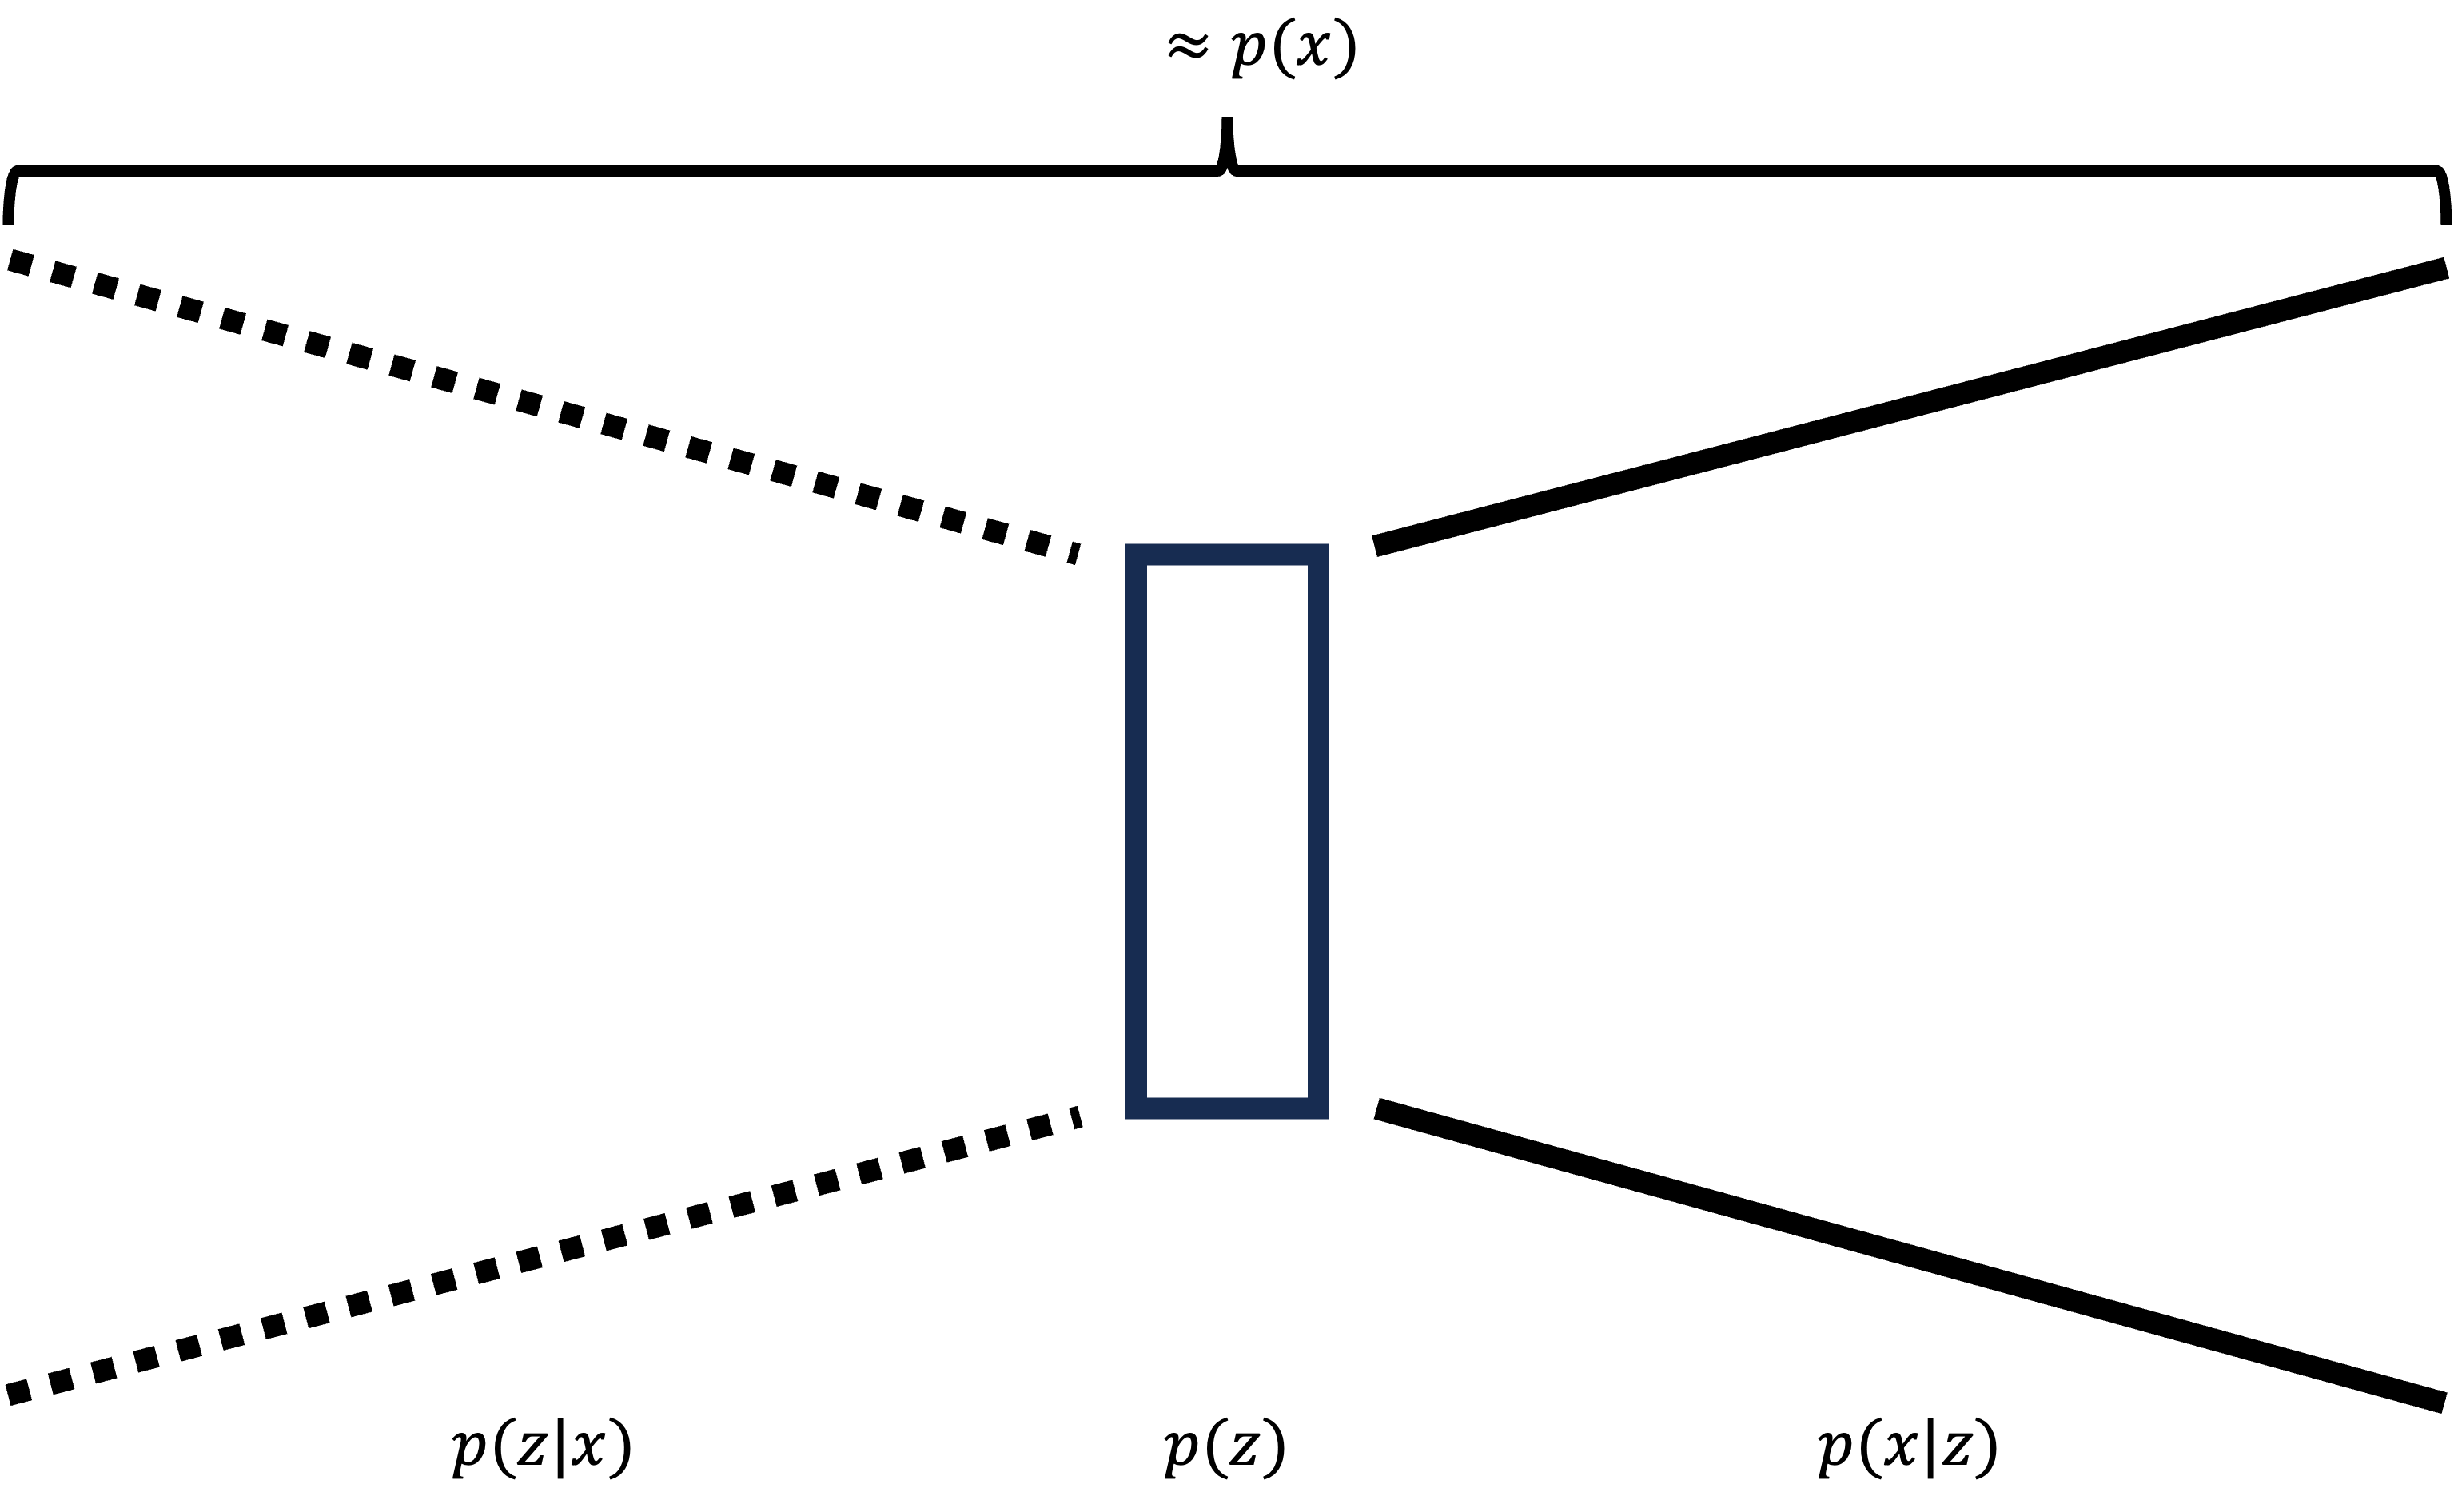
\includegraphics[width=.5\textwidth]{images/vae.png}
    \caption[VAE schematic]{VAE schematic: $p(x)$ is approximated through a latent variable model where posterior and likelihood are modeled with neural networks and the prior on the latent variable is modeled through a simple parameterized distribution (often Gaussian). The hope is, that after training, sampling from $p(z)$ and passing it through the neural network $p_{\theta_{NN}}(x|z)$, is the same as sampling from $p(x)$.}
    \label{fig:vae}
\end{figure}
Figure
The name of the VAE stems from the Autoencoder, a neural network that learns to recreate its output through an encoder with a bottleneck and a decoder, thereby learning a compressed representation of the data at the bottleneck and Fig.~\ref{fig:vae} illustrates the connection.~\autocite{https://doi.org/10.1002/aic.690370209} Autoencoders bear similarity to other dimension reduction methods like Principal Component Analysis (PCA) and therefore were first published under the name \textit{Nonlinear principal component analysis}.
\subsection{KL Divergence and Variational Lower Bound}
In VAEs, the encoder $p_{\theta}(z|x)$ needs to approximate the true posterior $p(z|x)$ and sampled data should look like it was sampled from $p(x)$. This requires a measure that can compare the similiarity between two probability distributions. One such heavily used measure is the KL (Kullback-Leibler) divergence, formulated for the posterior and its approximation as
\begin{equation}
    \label{eq:kldivergence}
    KL\left[p_{\theta}(z|x) || p(z|x)\right] = \int \log \frac{p_{\theta}(z|x)}{p(z|x)} p_{\theta}(z|x) dz = \mathbb{E}_{z\sim p_{\theta}(z|x)}\left[\log \frac{p_{\theta}(z|x)}{p(z|x)}\right].
\end{equation}
The KL divergence has the properties of being strictly non-negative and only being 0 if the two distributions are equal, but the proofs of those properties are omitted in this work.

The problem with the KL divergence in Eq.~\ref{eq:kldivergence} is that the true posterior is unknown. We will therefore introduce a loss function called ELBO (evidence lower bound) or VLB (variational lower bound) that automatically makes sure that the KL divergence between the parameterized posterior and the true posterior is minimized, without knowing $p(z|x)$. For understanding the ELBO, it is important to note that the marginal log-likelihood can be written as follows (derivation in the appendix):
\begin{align}
    \log p_{\theta}(x) & = \mathbb{E}_{z\sim p_{\theta_{NN}}(z|x)}\left[\log \frac{p_{\theta_{NN}}(x|z) p_{\theta_z}(z)}{p_{\theta_{NN}}(z|x)}\right] + KL\left[p_{\theta_{NN}}(z|x)||p(z|x)\right]
\end{align}
From the properties of the KL divergence we know that the second term on the right hand side is strictly non-negative, this means that the first term on the right hand side offers a lower bound to the log-likelihood of the data and the difference between that first term and the log-likelihood of the data is exactly the KL divergence that we wanted to minimize in Eq.~\ref{eq:kldivergence}. The relationship is also illustrated in Fig.~\ref{fig:elbo}.
\begin{equation}
    \label{eq:elbo}
    \log p_{\theta}(x) \geq \mathbb{E}_{z\sim p_{\theta_{NN}}(z|x)}\left[\log\frac{p_{\theta_{NN}}(x|z) p_{\theta_z}(z)}{p_{\theta_{NN}}(z|x)}\right]
\end{equation}
\begin{figure}[h]
    \centering
    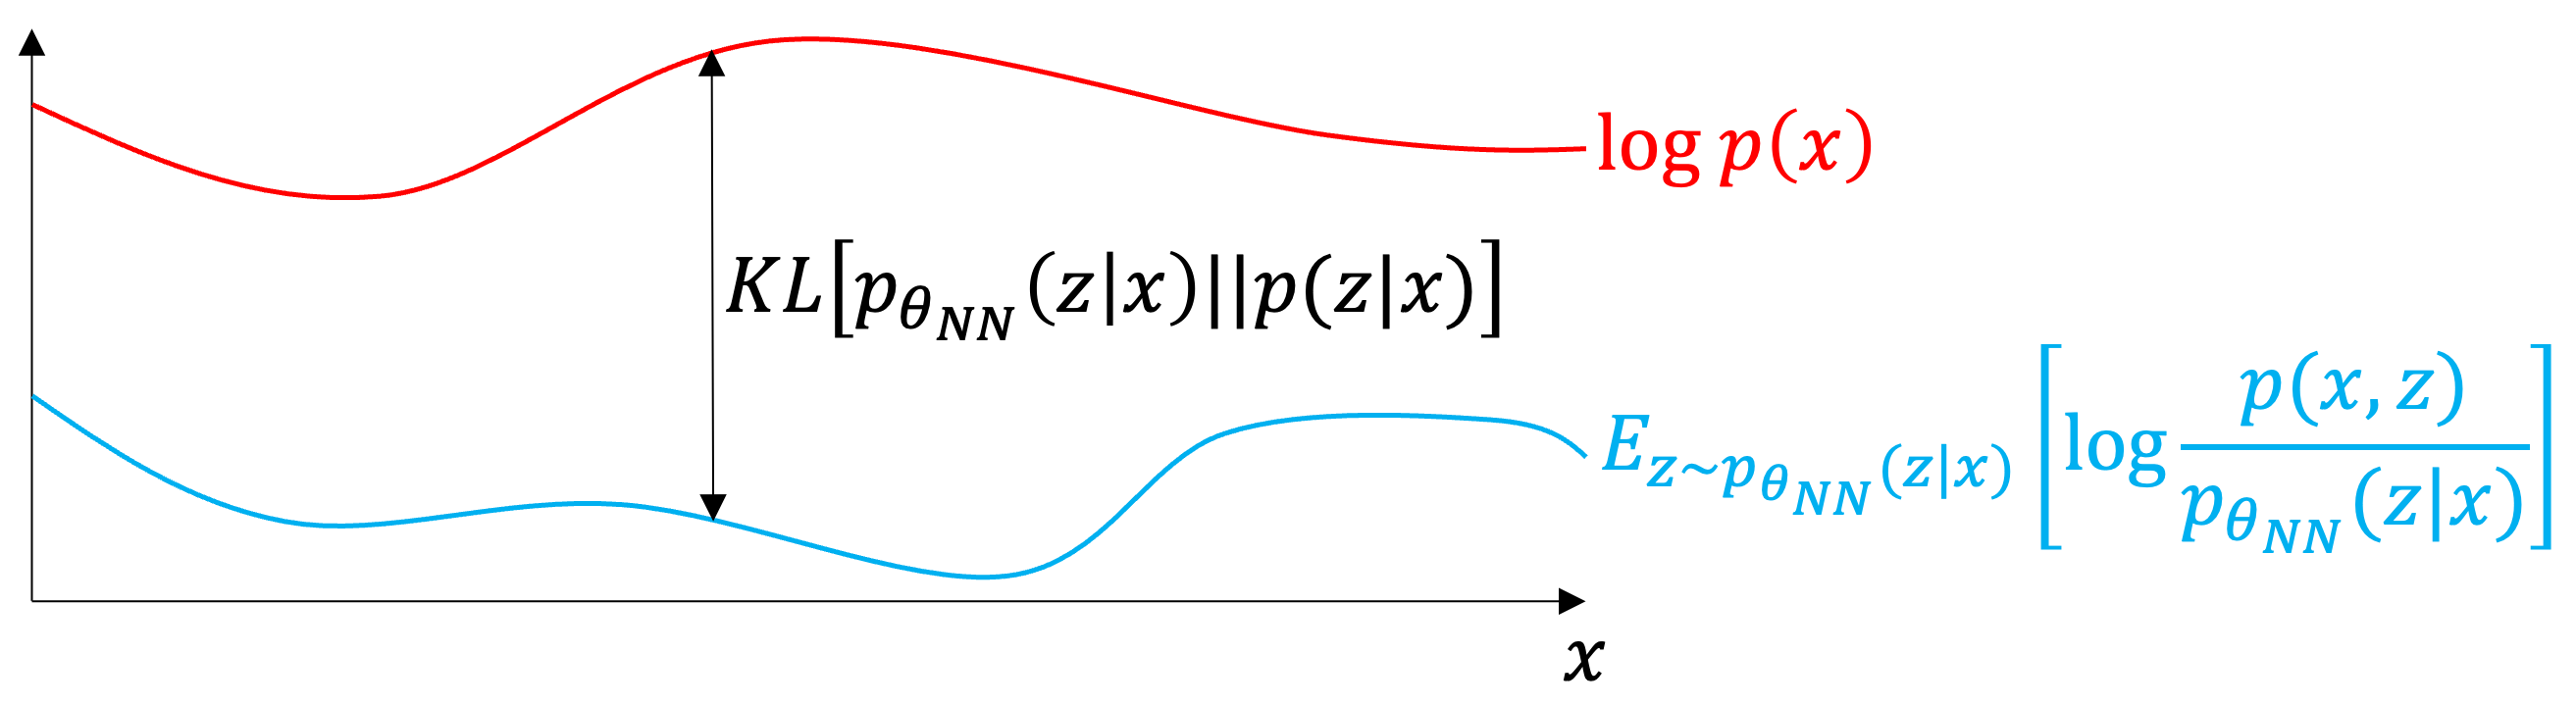
\includegraphics[width=.5\textwidth]{images/elbo.png}
    \caption[Illustration of the ELBO/VLB]{Illustration of the ELBO/VLB: The ELBO term gives a lower bound to the log-likelihood since the KL divergence is strictly non-negative. By maximizing the ELBO term, the KL divergence term is implicitly minimized and ELBO term converges towards the log-likelihood.}
    \label{fig:elbo}
\end{figure}
This means that, if we could maximize the term ELBO term from Eq.~\ref{eq:elbo} it would not only approach the log-likelihood, but simultaneously make sure that the estimated posterior converges to the true posterior. Luckily, for the parameterization of the VAE, the ELBO term can be split into two interpretable parts for optimization.
\begin{align}
    \mathbb{E}_{z\sim p_{\theta_{NN}}(z|x)}\left[\log\frac{p_{\theta_{NN}}(x|z) p_{\theta_z}(z)}{p_{\theta_{NN}}(z|x)}\right] & = \mathbb{E}_{z\sim p_{\theta_{NN}}(z|x)}\left[\log p_{\theta_{NN}}(x|z)\right] - \mathbb{E}_{z\sim p_{\theta_{NN}}(x|z)}\left[\log \frac{p_{\theta_{z}}(z)}{p_{\theta_{NN}}(z|x)}\right]                                        \\
                                                                                                                              & = \underbrace{\mathbb{E}_{z\sim p_{\theta_{NN}}(z|x)}\left[\log p_{\theta_{NN}}(x|z)\right]}_{\text{reasonable reconstruction}} - \underbrace{KL \left[p_{\theta_{NN}}(z|x)||p_{\theta_{z}}(z)\right]}_{\text{correct encoding}}
\end{align}
Maximizing the first part makes sure that the decoder reconstructs reasonable samples from the latent distribution, minimizing the second makes sure that the encoder transforms the training data into our chosen prior over the latents $z$ (usually Gaussian, as mentioned before). The reconstruction term is trivially maximized by minimizing some loss between input and output and if the prior $p(z)$ is chosen to be a Gaussian $p_{\theta_{z}}(z)$, then the KL divergence has a closed form, the derivation of which is omitted.~\autocite{mreasykldivergence}
\begin{equation}
    D_{KL}(p||q) = \frac{1}{2}\left[\log\frac{|\Sigma_q|}{|\Sigma_p|} - k + (\boldsymbol{\mu_p}-\boldsymbol{\mu_q})^T\Sigma_q^{-1}(\boldsymbol{\mu_p}-\boldsymbol{\mu_q}) + tr\left\{\Sigma_q^{-1}\Sigma_p\right\}\right]
\end{equation}

In the next section, the DDPM (diffusion denoising probabilistic model) will be introduced, which is the model architecture used throughout this work. As will be clear shortly, DDPMs can be viewed as a chained VAE that uses a sequence of latent spaces. This is an arguably easier learning problem, since the neural network does not have to map directly from noise to samples, but can do so in an iterative process over many steps.

\section{Diffusion Denoising Probabilistic Models}
Diffusion Denoising Probabilistic Models (DDPMs or Diffusion Models) are a generative model that learn the distribution of images in a training set. During training, sample images are gradually destroyed by adding noise over many iterations and a neural network is trained, such that these steps can be inverted.

As the name suggests, image content is diffused in timesteps, therefore we use the random variable $\bm{x}_0$ to represent our original training images, $\bm{x}_t$ for (partially noisy) images at an intermediate timestep and $\bm{x}_T$ for images at the end of the process where all information has been destroyed, and the distribution $q(\bm{x}_T)$ largely follows an isotropic Gaussian distribution.

The goal is to train a network that creates a less noisy image $\bm{x}_{t-1}$ from $\bm{x}_t$. If this is achieved over the whole training distribution, then sampling new $\bm{x}_T$ and passing and iteratively denoising it, should be the same as sampling $q(\bm{x}_0)$ directly.

\subsection{Forward Diffusion Process}
In order to derive a training objective it is important to understand the workings of the \textit{forward diffusion process}. During this process, i.i.d (independent and identically distributed) Gaussian noise is applied to the image over many discrete timesteps. A \textit{variance schedule} defines the means and variances ($\sqrt{1-\beta}$ and $\beta$) of the added noise at every timestep.~\autocite{ho2020denoising} The whole process can be expressed as a Markov chain (depicted in Fig.~\ref{fig:forward_diffusion}), with the factorization
\begin{align}
    \label{eq:forwardprocess}
    q(\bm{x}_{0:T})            & = q(\bm{x}_0) \prod_{t=1}^{T} q(\bm{x}_{t}|\bm{x}_{t-1}) &  & \text{(joint distribution)}       \\
    q(\bm{x}_{0:T}|\bm{x}_{0}) & = \prod_{t=1}^{T} q(\bm{x}_{t}|\bm{x}_{t-1})             &  & \text{(forwarding single sample)}
\end{align}
where the transition distributions $q(\bm{x}_t|\bm{x}_{t-1}) = \mathcal{N}(\sqrt{1-\beta_t} \bm{x}_{t-1}, \beta_t I)$ and we used the shorthand notation $\bm{x}_{0:T} = \bm{x}_{0},\dots,\bm{x}_{T}$. An example of iterative destruction of an image by this process is shown in Fig.~\ref{fig:forward_naoshima}.

\begin{figure}[h]
    \centering
    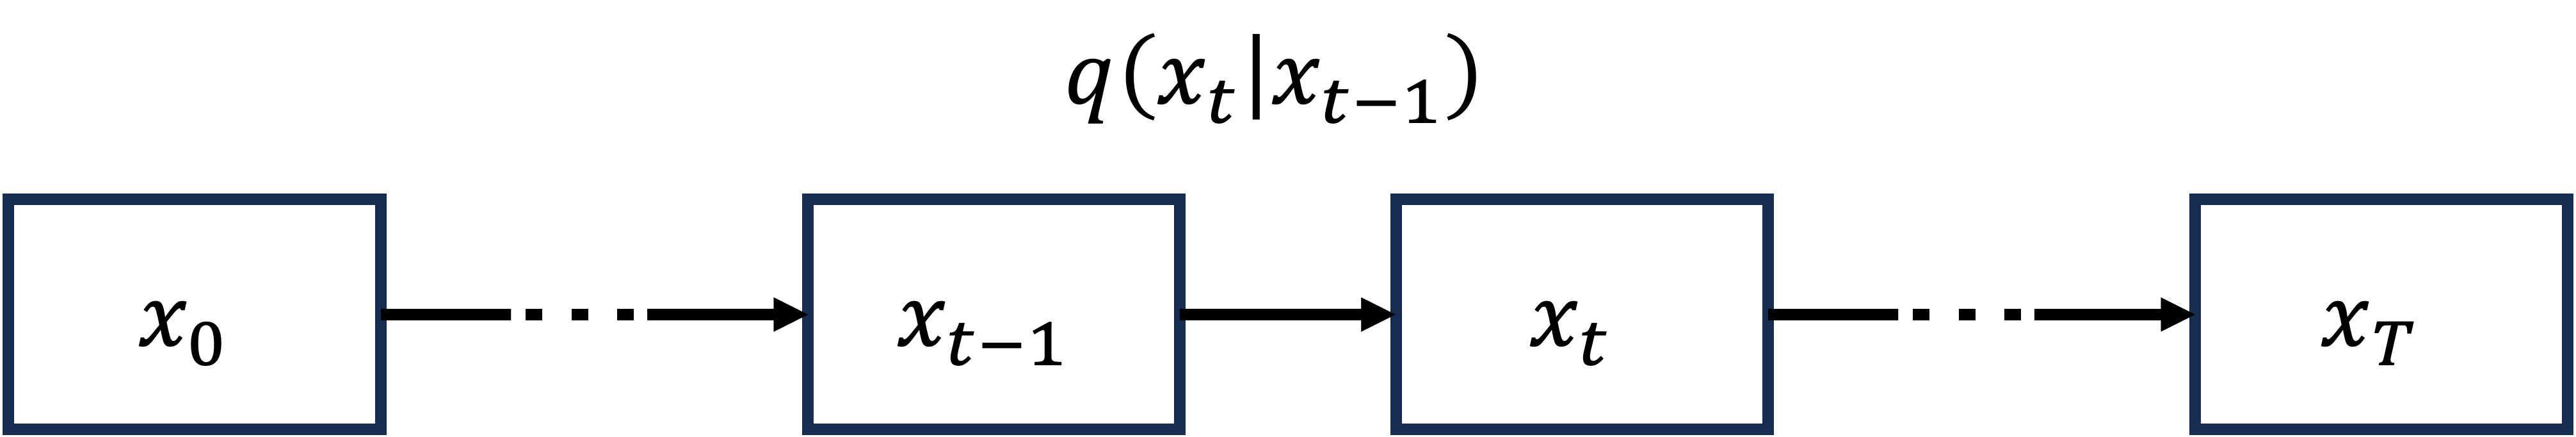
\includegraphics[width=.5\textwidth]{images/forward_diffusion.png}
    \caption[Markov Chain Interpretation of Forward Diffusion Process]{Markov Chain Interpretation of Forward Diffusion Process: An image is iteratively destroyed by adding normally distributed noise,
        according to a schedule. This represents a Markov process with the transition probability $q(\bm{x}_t|\bm{x}_{t-1})$.}
    \label{fig:forward_diffusion}
\end{figure}

\begin{figure}[h]
    \centering
    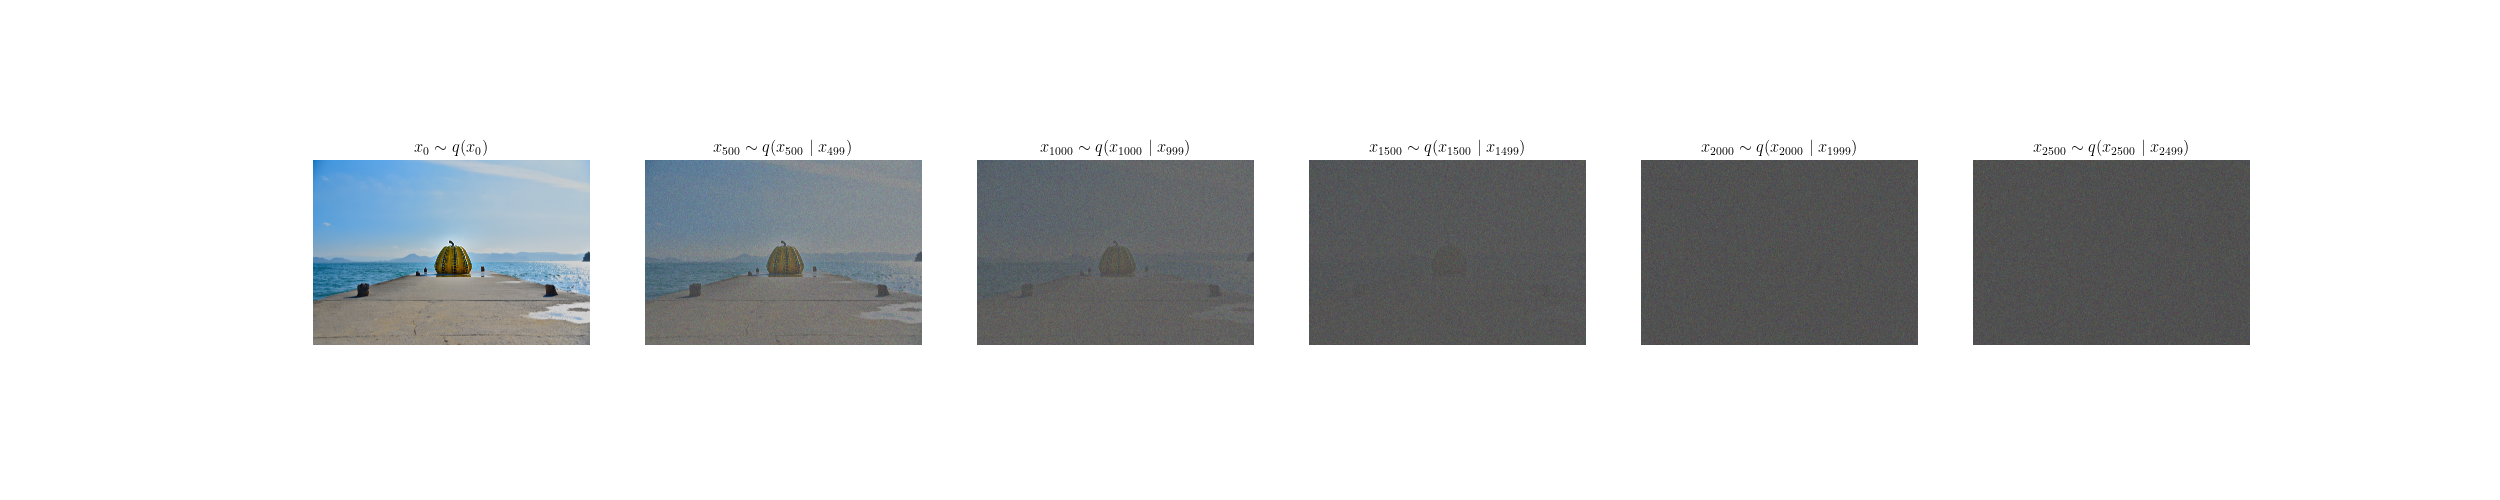
\includegraphics[width=\textwidth]{images/forward_naoshima.png}
    \caption[Example of Iterative Image Destruction through Forward Diffusion Process]{Example of Iterative Image Destruction through Forward Diffusion Process:
        The indices give the time step in the iterative destruction process, where $\beta$ was created according to a linear noise variance schedule (5000 steps from in the 0.001 to 0.02 range and picture resolution of 4016$\times$6016 pixels).}
    \label{fig:forward_naoshima}
\end{figure}

Gladly it is not necessary to sample noise again and again in order to arrive at $\bm{x}_t$, since Ho et al. derived a closed-form solution to the sampling procedure.~\autocite{ho2020denoising} For this, the variance schedule is first reparameterized as $1-\beta = \alpha$
\begin{equation}
    q(\bm{x}_t | \bm{x}_{t-1}) = \mathcal{N}(\sqrt{\alpha_t} \bm{x}_{t-1}, (1-\alpha_t) \bm{I})
    \label{eq:forward_alpha}
\end{equation}
and the closed-form solution for $q(\bm{x}_t|\bm{x}_0)$ is derived by introducing the cumulative product $\bar{\alpha}_t = \prod_{s=1}^{t}\alpha_s$ as
\begin{equation}
    q(\bm{x}_t|\bm{x}_0) = \mathcal{N}(\sqrt{\bar{\alpha}_t}\bm{x}_0, (1-\bar{\alpha}_t)\bm{I})
    \label{eq:forward_alphadash}
\end{equation}
The derivation that leads from Eq.~\ref{eq:forward_alpha} to Eq.~\ref{eq:forward_alphadash} is left to appendix~\ref{app:forward}.

A choice of $\bar{\alpha}_t \in [0,1]$ in above parameterizaiton ensures that the variance does not explode in the process, but that the SNR (signal-to-noise-ratio) still goes to 0 by gradually attenuating the means, corresponding to the original image. Thanks to the reparameterization with $\bar{\alpha}_t$, the forward process is also not restricted anymore to discrete timesteps, but a continuous schedule can be used.~\autocite{kingma2023variational,song2021scorebased}

The process of information destruction is dependent on the chosen variance schedule, the number of steps and the image size. Beyond the most simple case -- a constant variance over time -- Ho et al. opted for the second most simple option, a linear schedule, where the variance $\beta_t$ grows linearly in $t$.~\autocite{ho2020denoising} Nichol et al. later found that a cosine-based schedule gives better results on lower resolution images, since it does not destruct information quite as quickly, making it more informative in the last few timesteps. They also mention that their cosine schedule is purely based on intuition and they expect similar functions to perform equally well.~\autocite{nichol2021improved}  Own experiments exploring above mentioned parameters are explained in~\ref{sec:forward_diff_experiments} and plots of the two different variance schedules are visible in Fig.~\ref{fig:alphadash}.

\subsection{Reverse Diffusion Process}
As mentioned before DDPMs can be viewed as latent space models in a similar way that Generative Adversarial Nets or Variational Autoencoders can.~\autocite{goodfellow2014generative,kingma2013autoencoding} In DDPMs the reverse process is essentially again a Markov chain and can therefore again be factorized as
\begin{equation}
    \label{eq:reverseprocess}
    q(\bm{x}_{0:T}) = q(\bm{x}_T) \prod_{t=T}^{1} q(\bm{x}_{t-1}|\bm{x}_{t})
\end{equation}
where we start from $\bm{x}_T\sim\mathcal{N}(0,\bm{I})$. This means that the network does not learn to approximate the full inversion, but rather just the transition probabilities $q(\bm{x}_{t-1}|\bm{x}_{t})$ in the chain, which are transitions between several intermediate latent distributions. During training, we will need to condition the inversion on a training sample, where the Markov properties of the reverse process will no longer hold. In the appendix, it is shown that the inversion is also Gaussian, we therefore train a neural network to approximate
\begin{equation}
    \label{eq:reverseapprox}
    q(\bm{x}_{t-1} | \bm{x}_t) \approx p_{\theta}(\bm{x}_{t-1} | \bm{x}_t) = \mathcal{N}(\bm{\mu}_{\theta}(\bm{x}_t, t),\bm{\Sigma}_{\theta}(\bm{x}_t, t)).
\end{equation}

\subsection{Loss Functions}
The combination of forward $q(\bm{x}_T|\bm{x}_0)$ and reverse process $q(\bm{x}_0|\bm{x}_T)$ can be viewed as a chain of VAEs and we can again formulate a variational lower bound objective like before. The lengthy derivation of the ELBO for the DDPM is omitted in this work, but can be looked up in the Calvin Luo's work.~\autocite{luo2022understanding} The final form is similar to the one from the VAE, with a reconstruction term and a prior matching term, but with additional terms that match the intermediate latents.
\begin{align}
    \log p_{\theta}(x) & \geq \underbrace{\mathbb{E}_{q(x_1|x_0)} \left[ \log p_{\theta}(x_0|x_1) \right]}_{\text{reasonable reconstruction}}          \\
                       & - \underbrace{KL \left[ q(x_T|x_0) || p(x_t) \right]}_{\text{correct encoding}}                                               \\
                       & - \sum_{t=2}^{T} \underbrace{KL \left[ q(x_{t-1}|x_{t},x_0) || p_{\theta}(x_{t-1}|x_{t}) \right]}_{\text{denoising matching}}
\end{align}
The term $q(x_{t-1}|x_{t},x_0)$ is the true reverse process, conditioned on a single sample. This term comes to be when substituting the posterior transitions $p(x_t|x_{t-1})$ with $p(x_t|x_{t-1}, x_0)$, which is allowed since the Markov property states that $x_t$ only depends on $x_{t-1}$. The natural choice for the denoising matching term would be $KL\left[ q(x_t|x_{t-1}) || p_{\theta}(x_t|x_{t+1}) \right]$, but this has higher variance and is therefore harder to estimate.~\autocite{ho2020denoising} Due to the DDPM usually having 1000 or more timesteps, the ELBO is dominated by the third term. For this reason the first term is usually not used during optimization, since it can only be estimated using Monte Carlo sampling. While it is not used for optimization, it can be useful for evaluating the performance of a trained model. The second term is parameter-free therefore also not used for optimization. It should anyway be zero if the parameterization of the forward process is correct, which means that forward diffused samples get close to our chosen latent prior $p(x_T) = \mathcal{N}(0,\bm{I})$. As mentioned before, $p_{\theta}(x_{t-1}|x_t)$ is also Gaussian and since it was decided to fix the variances of the transitions to a fixed schedule, the variances of the inversion are often fixed as well and only the means are learned. When looking at the formula for the KL divergence between two Gaussians (Eq.~\ref{eq:kldivergence}) with fixed diagonal covariance matrices, one can derive that it reduces to a mean squared error between the distributional means.~\autocite{luo2022understanding}
\begin{equation}
    \hat{\theta} = \argmin_{\theta} KL \left[ q(x_{t-1}|x_{t},x_0) || p_{\theta}(x_{t-1}|x_{t}) \right] = \argmin_{\theta} \frac{1}{2\beta(t)^2} \left[ || \mu_{\theta} - \mu_{q} ||_2^2 \right]
\end{equation}
Ho et al.~\autocite{ho2020denoising} found that it works best, if the network is trained to predict the noise in the image directly and the means are then found through reparameterization
\begin{equation}
    \mu_{\theta}(x_t,t) = \frac{1}{\sqrt{\alpha_t}}x_t - \frac{1-\alpha_t}{\sqrt{1-\bar{\alpha}_t}\sqrt{\alpha_t}}\hat{\epsilon}_{\theta}(x_t,t)
\end{equation}
which transforms the loss from before into
\begin{equation}
    \hat{\theta} = \argmin_{\theta}\frac{1}{2\beta(t)^2} \frac{(1-\alpha_t)^2}{(1-\bar{\alpha}_t)\alpha_t} \left[ || \epsilon_0 - \hat{\epsilon}(x_t, t)  ||_2^2 \right]
\end{equation}


Another simplification is usually taken and $p_{\theta}(\bm{x}_{t-1} | \bm{x}_t)$ only approximates the means $\bm{\mu}_{\theta}$ and not the variances. For small enough timesteps, the means determine the transitional distributions much stronger than the variances. The network is furhter usually trained to not predict the means directly, but the noise and the means are then determined through a reparameterization.~\autocite{ho2020denoising,nichol2021improved}

\section{Guided Diffusion}
\subsection{Classifier Guidance}
Classifier guidance as termed by Nichol et al. introduces a data consistency term $p(s|x_t)$ in the form of a classifier trained on noisy images, where $s$ is the random variable expressing if an image belongs to a certain class.~\autocite{dhariwal2021diffusion,sohldickstein2015deep} Conditioning on a classifier is sucessfully used by taking gradient ascent steps not only in the direction that maximizes the prior $p(x)$ in a DDPM $\nabla_{x_t} \log p(x_t)$, but also the direction of this conditioning term $\nabla_{x_t} \log p(s|x_t)$. In total, this is equal to Eq.~\ref{eq:mapestimation}
\begin{equation}
    x_{t+1} = \underbrace{x_{t} + \nabla_{x_t} \log p(x_t)}_{x'_{t+1}} + \lambda \nabla_{x_t} \log p(s|x_t)
\end{equation}
with $x'_{t+1}$ being the prediction of the reverse diffusion steps before any conditioning and $\lambda$ an arbitrary factor determining the strength of the guidance.

\subsection{Image-Guided Diffusion}
\label{sec:imageguidance}
Knowledge of the forward process makes it possible to inject information from target images into the latent space where they can be fused with prediction. Lugmayr et al. make use of this for the tasks of image inpainting by always substituting the known image areas during the reverse diffusion.~\autocite{lugmayr2022repaint}
\begin{equation}
    x_{t} = \mathcal{M}^{-1}(x_t) + \mathcal{M}(s_t)
\end{equation}
They further enhance their approach using a resampling strategy, that gives the model more time to harmonize the semantics of the image. An example of such a resampling schedule can be seen in Fig.~\ref{fig:stepsplot}.

Choi et al. also substitute parts of the image in order to guide the inverse diffusion process, but they substitute low-frequency information by using linear filters.~\autocite{choi2021ilvr}
\begin{equation}
    x_{t} = \phi(s_{t}) + (I - \phi) (x_{t})
\end{equation}
They demonstrate strong performance in image translation tasks, e.g. from painting to photo-realistic image.